\clearpage
\sloppy
\chapter{THUẬT TOÁN SVM VỚI ÁNH XẠ ĐẶC TRƯNG TUYẾN TÍNH TỪNG PHẦN}
\section{Thuật toán SVM (Support Vector Machine)}
\textit{SVM} là một thuật toán học máy có giám sát được sử dụng cho các tác vụ phân loại và hồi quy. SVM hoạt động bằng cách tìm một siêu phẳng trong không gian nhiều chiều để phân loại dữ liệu thành các lớp khác nhau. SVM có thể xử lý cả các vấn đề phân loại tuyến tính và phi tuyến tính bằng cách sử dụng các đặc trưng \textit{hạt nhân - kernel} khác nhau. Nó được sử dụng rộng rãi trong các tác vụ như phân loại hình ảnh, phân loại văn bản, \(\dotsc\)

\begin{figure}[htbp]
    \centering
    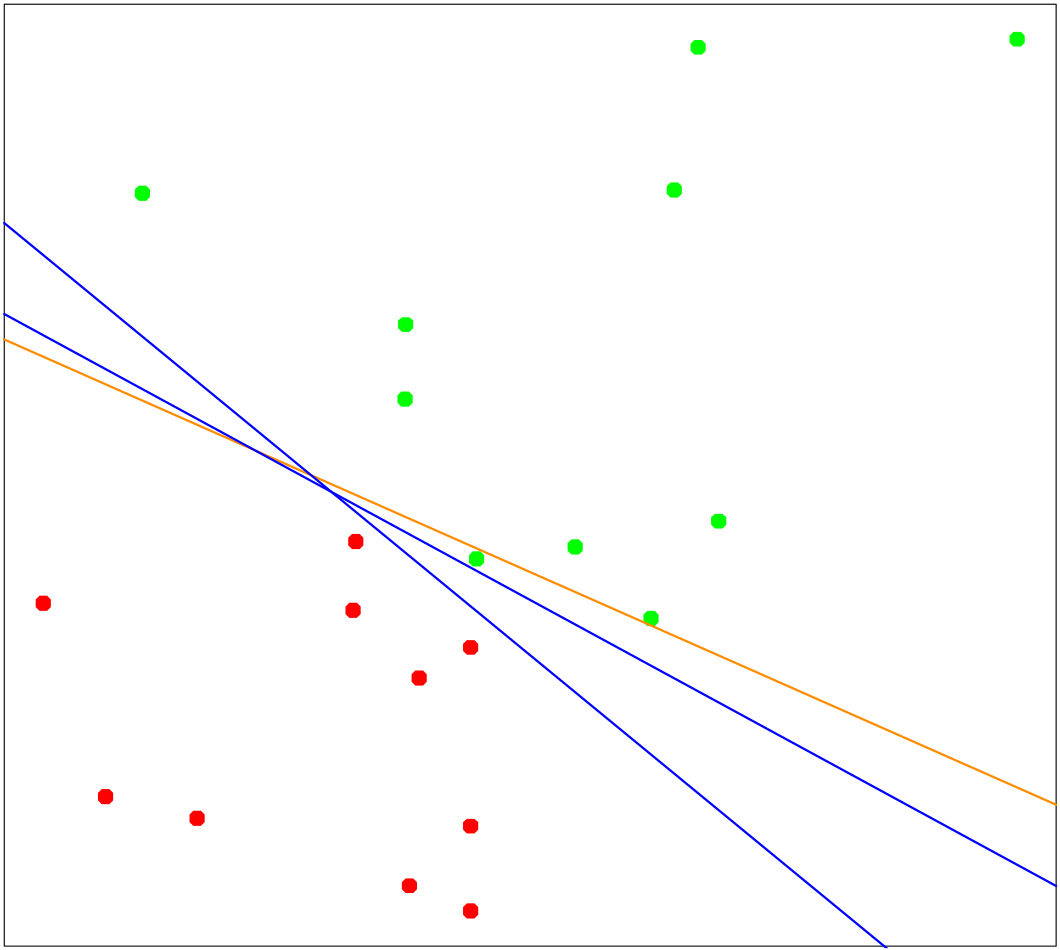
\includegraphics[width=0.6\textwidth]{images/separate_hyper_example.png}
    \caption[Minh họa siêu phẳng phân tách]{Một ví dụ với hai lớp có thể phân tách bằng siêu phẳng. Đường màu cam là nghiệm bình phương tối thiểu, phân loại sai một trong các điểm huấn luyện. Ngoài ra còn có hai siêu phẳng phân tách màu xanh được tìm thấy bởi thuật toán học perceptron với các điểm khởi đầu ngẫu nhiên khác nhau.}
    \label{fig:separate_hyper_example}
\end{figure}

\noindent Xét bài toán phân chia hai lớp dữ liệu, giả sử rằng có hai lớp dữ liệu được mô tả bởi các điểm (véctơ đặc trưng) trong không gian nhiều chiều, hơn nữa, hai lớp dữ liệu này là có thể phân tách tuyến tính, tức là tồn tại một siêu phẳng phân chia chính xác hai lớp đó. Hãy tìm một siêu phẳng phân chia hai lớp đó, tức tất cả các điểm thuộc một lớp nằm về cùng một phía của siêu phẳng đó và ngược phía với toàn bộ các điểm thuộc lớp còn lại. Hình \ref{fig:separate_hyper_example} cho ta ví dụ về vô số nghiệm (tức đường thẳng phân chia) cho bài toán phân loại trên.

\begin{figure}[htbp]
    \centering
    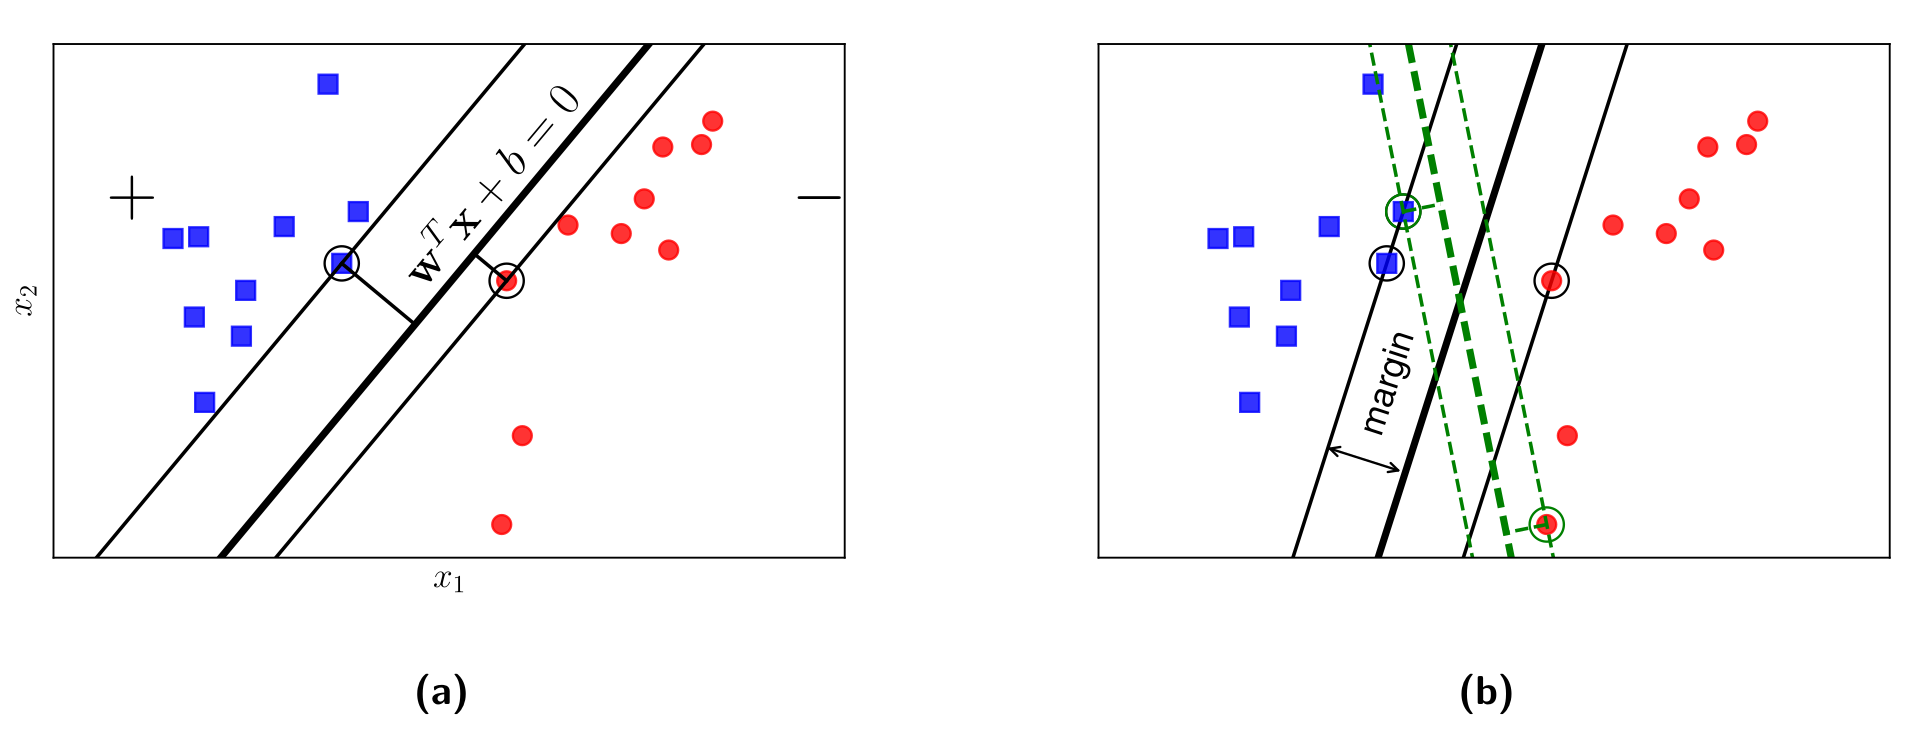
\includegraphics[width=\textwidth]{images/svm_introduce.png}
    \caption[Ý tưởng của SVM]{\textit{Lề (Margin)} của một lớp được định nghĩa là khoảng cách từ các điểm gần nhất của lớp đó tới mặt phân chia. \textbf{(a)} Minh họa về một phân loại chưa tốt khi khoảng cách từ điểm màu đỏ tới mặt phân chia là ngắn hơn. \textbf{(b)} Minh họa về một phân loại tốt (đường màu đen liền nét) với các điểm màu xanh và đỏ nằm ở hai bên mặt phân chia, và lề của hai lớp là bằng nhau.}
    \label{fig:svm_introduce}
\end{figure}

\subsection{Xây dựng bài toán tối ưu cho SVM}
Giả sử rằng các cặp dữ liệu trong tập huấn luyện là $(\mathbf{x}_1, y_1)$, $(\mathbf{x}_2, y_2)$, $\dotsc$, $(\mathbf{x}_n, y_n)$ với véctơ $\mathbf{x}_i \in \R^d$ thể hiện đầu vào của một điểm dữ liệu và $y_i$ là nhãn của điểm dữ liệu đó, $d$ là số chiều của dữ liệu và $n$ là số điểm dữ liệu. Giả sử rằng nhãn của mỗi điểm dữ liệu được xác định bởi $y_i = 1$ hoặc $y_i = -1$. Thêm nữa, giả sử mặt phân chia có phương trình là $\mathbf{w}^T\mathbf{x} + b = 0$, với cặp dữ liệu $(\mathbf{x}_n, y_n)$ bất kỳ, khoảng cách từ điểm đó tới mặt phân chia là:
\begin{equation}
    \frac{y_n(\mathbf{w}^T\mathbf{x}_n + b)}{\|\mathbf{w}\|_2},
\end{equation}

\noindent Từ đó, lề (margin) của mặt phân chia được định nghĩa là khoảng cách từ điểm gần nhất tới mặt phân chia (tính ở cả hai lớp), tức là:
\begin{equation}
    \min_{n} \frac{y_n(\mathbf{w}^T\mathbf{x}_n + b)}{\|\mathbf{w}\|_2},
\end{equation}

\noindent Bài toán tối ưu của SVM tức là tìm \(\mathbf{w}\) và \(b\) sao cho lề đạt giá trị lớn nhất:
\begin{equation}
    \arg \max_{\mathbf{w}, b} \left\{ \min_{n} \frac{y_n(\mathbf{w}^T\mathbf{x}_n + b)}{\|\mathbf{w}\|_2} \right\},
\end{equation}

\noindent Có thể thấy rằng nếu thay véctơ hệ số $\mathbf{w}$ bởi $k\mathbf{w}$ và $b$ bởi $kb$ với $k > 0$ thì mặt phân chia không thay đổi. Do đó, ta có thể giả sử rằng với những điểm nằm gần mặt phân chia nhất, ta có:
\begin{equation}
    y_n(\mathbf{w}^T\mathbf{x}_n + b) = 1
\end{equation}
Như vậy, với mọi \(n\) ta luôn có: \(y_n(\mathbf{w}^T\mathbf{x}_n+b)\geq 1\)

\noindent Do đó, bài toán tối ưu này có thể đưa về dạng
\begin{align}
    &\arg \min_{\mathbf{w}, b} \frac{1}{2}\|\mathbf{w}\|_2^2 \notag \\
    &\text{thỏa mãn: } 1 - y_n(\mathbf{w}^T\mathbf{x}_n + b) \leq 0, \forall n = 1, 2, \dotsc, n
\end{align}

\noindent Không mất tính tổng quát, ta có thể lấy nghịch đảo hàm mục tiêu, bình phương nó để được một hàm khả vi, và nhân với \(\frac{1}{2}\) để công thức đạo hàm đẹp hơn.

\subsection{Lề cứng (Hard margin) và lề mềm - (Soft margin)}